\section{Question 3}
    You are given a dataset of 3168 labeled instances for voice-based gender classification:\\
    \texttt{data\_gender\_voice.csv}. 
    Each instance contains 19 acoustic features extracted from voice recordings in the 0-280Hz frequency band. 
    The associated label is in the last column ofthe dataset, where `1' indicates male and `0' indicates female.

    \subsection{Item a}
    Perform a basic feature analysis: plot the histograms of the features and compute their correlations. 

    \subsection{Item b}
    Implement a logistic regression model to classify voice instances  by gender. 
    Use a 20\% split for the test set, with the remaining instances for training. 
    Keep in mind that the dataset is ordered, therefore, randomization is necessary before splitting. 
    Consider whether  preprocessing  (e.g. normalization)  is appropriate. 
    Present and discuss the results on the test set, including:
    %
    \begin{itemize}
        \item the ROC curve;
        \item the F1-score versus decision threshold curve.
    \end{itemize}
    %
    See Chapter 20 of the textbook and this \href{https://www.sciencedirect.com/science/article/abs/pii/S0306457309000259}{paper} for more information about the ROC curve and F1-score.
    
    \subsection{Item c}
    Which decision threshold is the most appropriate? 
    Why? 
    Using this threshold, compute and plot the confusion matrix and the classifier accuracy on the test set.
    Discuss your results.
    
\noindent\rule{\textwidth}{.5pt}

Assuming that a collection of samples' classes follow gaussian distributions, 
a standard Bayesian approach would use a subset of the original dataset
(i.e., the \textit{training} dataset) 
to first estimate each of these underlying distributions' parameters
(e.g., covariance matrix),
as well as prior probabilities of each distribution, 
to tune a discriminant function.
%
Then, with a subset from the original samples different than the training set (i.e., the \textit{test} set),
the discriminant is applied sample by sample and its results, 
the degree of belief that the sample belongs to a class,
compared with the associated original classification.

The logistic regression, as in the Bayesian approach, 
assumes there are underlying gaussian distributions to the classifications,
but the algorithm circumvents the parameter estimations by
bringing the analysis straight to the data,
weighting the attributes influences on the classifications.
%
In particular, the logistic regression assumes that classes 
can be separated by lines in feature space, making the weighting linear.

This discussion merits mathematical detailing.
%
Let:
\begin{itemize} 
    \item $N$ be the number of samples;
    \item $K$ be the number of different classes a sample can assume;
    \item $d$ be the number of attributes;
    \item $\mathbf{x}_i$, a $1\times d$ row vector, be the $i$-th sample;
    \item $\mathbf{X}_{N\times d}$ be the original dataset.  
\end{itemize}
%
The discriminant associated with class $k$ applied to sample $\mathbf{x}_i$  
is denoted by $b_{ki}$ and given by 
%
\begin{equation}
    b_{ki} = \mathbf{w}_k[1\quad \mathbf{x}_i]^\text{T},
    \quad
    1\leq k\leq K
    \label{eq:b_ki}
\end{equation}
%
where $\mathbf{w}_k = [w_0\ w_1\ \dots\ w_d]$ is a $1\times (d+1)$ row vector 
whose entries correspond to the weight of each attribute in leading to class $k$
(plus a term $w_0$ for the line's linear coefficient).
%
Then, the probability that sample $i$ belongs to class $k$ is denoted by $y_{ki}$ and given by%
\footnote{
    This operation is also called softmax.
}%
%
\begin{equation}
    y_{ki} 
    = \frac{\exp(b_{ki})}
            {\exp(b_{1i}) + \exp(b_{2i}) + \dots + \exp(b_{Ki})}
    = \frac{\exp(b_{ki})}
           {\displaystyle\sum_{k=1}^K \exp(b_{ki})},
    \label{eq:y_ki}
\end{equation}

which can be shown to be equal to the posterior of class $k$ given sample $i$.
The associated original classifications are denoted by $r_{ki}$ and given by
%
\begin{equation}
    r_{ki} 
    = 
    \begin{cases} 
        1, &\mathbf{x}_i \text{ has class k} \\
        0, &\text{otherwise}
    \end{cases},
\end{equation}

to which the real-valued $\widehat{y}_{ki}$ is compared by ``snapping'' it to either $0$ or $1$,
according to a decision threshold $D$:
\begin{equation}
    y_{ki}^s = 
    \begin{cases} 
        1, &\widehat{y}_{ki} > D \\
        0, &\text{otherwise}
    \end{cases}.
    \label{eq:ys_ki}
\end{equation}
%
% and the error rate $E_\text{rate}$ of the regression becomes simply
% %
% \begin{equation}
%     E_\text{rate} = 
%     100\% \times
%     \frac{1}{NK} 
%     \sum_{i=1}^N 
%     \sum_{k=1}^K r_{ki} \odot y^s_{ki},
% \end{equation}
% %
% with $\odot$ representing the ``not xor'' operation 
% (i.e., 1 if arguments are equal and 0 otherwise).

Now, the most important part of the algorithm is how to tune the weight vectors $\mathbf{w}_k$.
In other words, there must be desgined a procedure to find 
$\mathbf{w}_k$ that maximizes the likelihood of $y_{ki}$.
Assuming the likelihood $r_{ki} | \mathbf{x}_i$ is Bernoulli$(y_{ki})$,
we have 
%
\begin{align}
    \mathbf{w}_k 
    &= 
    \argmax_{\mathbf{w}^*}
    \prod_{i=1}^N
    y_{ki}(\mathbf{w}^*)^{r_{ki}} \\
    &= 
    \argmin_{\mathbf{w}^*}
    -\sum_{i=1}^N
    r_{ki}\log(y_{ki}(\mathbf{w}^*)) \\ 
    &=
    \argmin_{\mathbf{w}^*} E_k(\mathbf{w}^*),
    \quad 
    E_k(\mathbf{w}^*) = 
    -\sum_{i=1}^N
    r_{ki}\log(y_{ki}(\mathbf{w}^*)).
    \label{eq:argmin}
\end{align}

One way of solving the minimization above is by using gradient-descent,
i.e., iteratively updating $\mathbf{w}^*$ with the gradient of the scalar function%
\footnote{
    Technically, this is the transpose of the gradient, which is given in column vector form.
}:
$\mathbf{w}^* \leftarrow \mathbf{w}^* - \eta\nabla E_k$.
%
Here, $\eta$ is a positive constant, called the learning rate, 
that regulates how far along the gradient direction the update must go. 
%
Given the relationships between $y_{ki}$, $b_{ki}$ and $\mathbf{w}_{ki}$ 
(equations \eqref{eq:b_ki}-\eqref{eq:y_ki}), one can show that 
%
\begin{align}
    \nabla E_k
    =
    -\sum_{i=1}^N 
    (r_{ki} - y_{ki}) 
    [1\quad \mathbf{x}_i].
    \label{eq:gradient}
\end{align}


The discussion above is nearly enough to derive an implementation of the logistic regression,
but a few points must still be addressed:
%
\begin{itemize}
    \item 
    First, since $b_{ki}$ is a weighted sum, attributes in greater ranges
    will have undue effect on the result. For that reason, it is important to normalize the data beforehand.

    \item 
    Second, gradient descent is only applied during training, 
    so $N$ in eqs. \eqref{eq:argmin} and \eqref{eq:gradient}
    becomes $N_\text{train} < N$.
    Usually, $0.7 \leq N_\text{train} / N \leq 0.8$.

    \item
    Third, there is no one best way of initializing $\mathbf{w}^*$ in the minimization.
    A simple way of doing so is taking random small values, say between $-0.01$ and $0.01$.
    Note that this range is reasonable only if data is normalized.

    \item 
    Fourth, the learning rate must be set. 
    Unless more advanced methods are used, e.g. line search and moving average,
    trial and error is required.

    \item
    Finally, the algorithm must have a stop condition.
    An epoch is a top-to-bottom reading of training set within the context of gradient descent.
    A simple way of finishing the descent, and thus the logistic discrimination,
    is to simply impose a limit on the number of epochs, $e_{\max}$.
\end{itemize}

The implementation of the logistic regression made here has set
$N_\text{train} = 0.8 N$, 
$\mathbf{w}^*$ entries initialized in $[-0.01, 0.01]$ (with seed of value $242104677$), 
$\eta = 0.1$ and $e_{\max} = 100$.
%
The learning rate and number of epochs were obtained through trial and error,
trying to make sure the algorithm finishes well into the elbow of the training error curve
while also having low error rates. 

The following is a pseudocode of the algorithm. 
Note that matrix multiplications have been used where convenient.
It was defined
%
\begin{align}
    \mathbf{W} &= 
    \begin{bmatrix}
        \mathbf{w}_1 \\ \mathbf{w}_2 \\ \vdots \\ \mathbf{w}_K
    \end{bmatrix}, 
\quad
    \mathbf{R} = 
    \begin{bmatrix}
        \mathbf{r}_1 \\ \mathbf{r}_2 \\ \vdots \\ \mathbf{r}_K
    \end{bmatrix}, 
\quad
    \mathbf{Y} = 
    \begin{bmatrix}
        \mathbf{y}_1 \\ \mathbf{y}_2 \\ \vdots \\ \mathbf{y}_K
    \end{bmatrix}
\end{align}
%
where
$\mathbf{r}_i = [r_{1i},\ r_{2i},\ \dots,\ r_{Ki}]$ and
$\mathbf{y}_i = [y_{1i},\ y_{2i},\ \dots,\ y_{Ki}]$.

\begin{algorithm}
    \caption{
        Implementation of the logistic regression (training). 
        Samples are assumed to be zero-mean and normalized.
    }
    \label{alg:logistic-regression}

    \KwData{$\mathbf{X}$, $\mathbf{R}$, $\eta$, $e_{\max}$}
    \KwResult{$\mathbf{Y}$, $\mathbf{W}$}

    $N \gets$ rows of $N$\;
    $d \gets$ columns of $N$\;
    $k \gets$ columns of $R$\;

    $\mathbf{W} \gets [\ \mathrm{random}(-0.01, 0.01)\ ]_{k\times d}$ 
    \Comment*[r]{Weights initially random}

    $epoch \gets 0$\;
    \While{%
        \text{epoch} $< e_{\max}$ 
    }{%
        $\mathbf{Y} \gets$ \texttt{calculate\_predictions}($\mathbf{W}, \mathbf{X}$) \Comment*[r]{Eqs. \eqref{eq:b_ki}, \eqref{eq:y_ki}}
        $\bm{\Delta}\mathbf{W} = 
        \displaystyle\sum_{i=1}^N 
            (\mathbf{r}_i-\mathbf{y}_i)^T 
            [1\quad \mathbf{x}_i]$
        \Comment*[r]{Opposite of gradient}
        $\mathbf{W} \gets \mathbf{W} + \eta\bm{\Delta}\mathbf{W}$ \Comment*[r]{Gradient descent}
        $epoch \gets epoch + 1$\;
    }
\end{algorithm}

\begin{algorithm}
    \caption{
        Class prediction calculation algorithm,
        with $\mathbf{u}_k$ the $k$-th row of $\mathbf{U}$.}

    \KwData{$\mathbf{W}$, $\mathbf{X}$}
    \KwResult{$\mathbf{Y}$}

    $N \gets$ rows of $\mathbf{X}$\;
    $K \gets$ columns of $\mathbf{W}$\;
    
    $\mathbf{B} \gets \mathbf{W}\ [\mathbf{1}_{N\times 1}\ \mathbf{X}]^\text{T}$ 
    \Comment*[r]{Matrix form of \eqref{eq:b_ki}}

    $\mathbf{U} \gets \exp.(\mathbf{B})$ 
    \Comment*[r]{Pointwise exponentiation of $\mathbf{B}$}

    $\mathbf{V} \gets \mathbf{1}_{k\times 1} \displaystyle\sum_{k=1}^K \mathbf{u}_k$ 
    \Comment*[r]{Broadcast of row sums}

    $\mathbf{Y} \gets \mathbf{U} ./ \mathbf{V}$ \Comment*[r]{Pointwise division, \eqref{eq:y_ki}}
\end{algorithm}

Before presenting the results of the logistic regression, 
a discussion on the dataset is necessary.
\cref{fig:correlations} presents the correlations between attributes, 
while \cref{fig:histograms} shows each attribute's histogram.

\begin{figure}[htbp]
    \centering
    \caption{
        Correlation between attributes as a colormap. 
        The original correlation matrix was reorganized as to 
        cluster bigger correlations at the upper left corner.
    }
    \label{fig:correlations}
    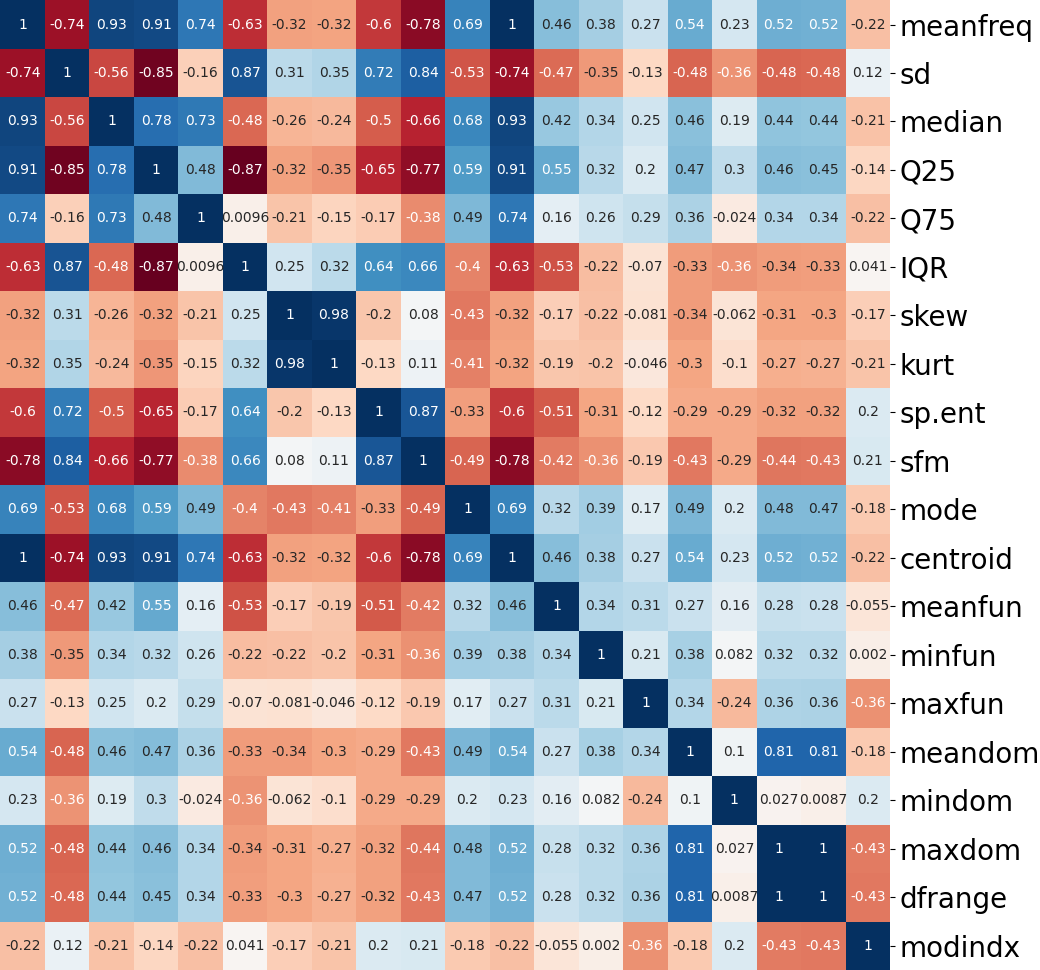
\includegraphics[width=.7\textwidth]
    {../../python_code/plots/logistic_regression/correlations.png}
\end{figure}

In training and testing, attributes with correlation greater than 0.95
were considered to add too little information to the sample, 
and thus removed from the dataset in order to simplify the arithmethic.
%
By inspecting \cref{fig:correlations},
one can see that, in all, three pairs of attributes are above the threshold.
%
Of those six, those removed were 
\texttt{meanfreq}, \texttt{kurt} and \texttt{maxdom}.
%
Indeed, \cref{fig:histograms} shows that the removed three are 
nearly identical to their pairs.

Having made it clear that the algorithm is now working with 
only 17 of the original 20 attributes, the results can be presented and discussed.
\cref{fig:weight-matrix} presents the weight matrix $\mathbf{W}$ obtained after training and used in testing.
%
Then,
\cref{fig:results-training} and 
\cref{fig:results-testing} 
show the F1-score and ROC for varying decision thresholds $D$ (see \eqref{eq:ys_ki}) 
obtained in training and testing, respectively.
%
\begin{figure}[htbp]
    \centering 
    \caption{
        Weight matrix as a colormap. 
        Bottom row classifies ``male'', top ``female''.
    }
    \label{fig:weight-matrix}
    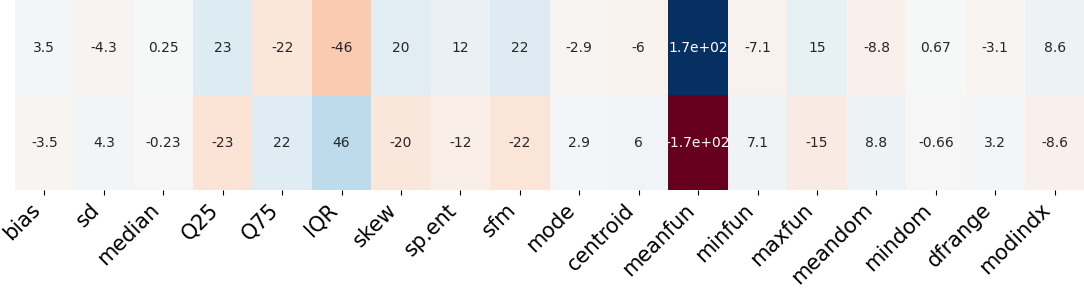
\includegraphics[width=.9\linewidth]{../../python_code/plots/logistic_regression/weight_matrix.png}
\end{figure}

\begin{figure}[htbp]
    \centering
    \caption{
        Histograms of attributes. 
        Highly correlated (removed) attributes were colored either orange, green or red.
    }
    \label{fig:histograms}
% First row
    \begin{subfigure}[t]{.24\textwidth}
        \centering 
        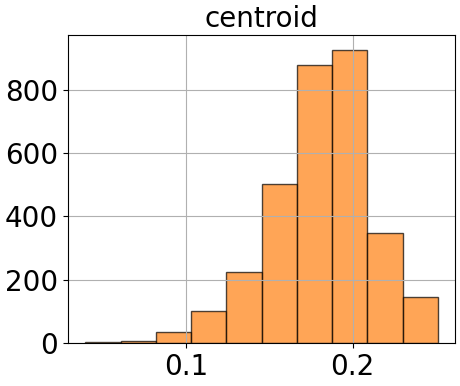
\includegraphics[width=\linewidth]{../../python_code/plots/logistic_regression/histogram-centroid.png}
    \end{subfigure}
    \begin{subfigure}[t]{.24\textwidth}
        \centering 
        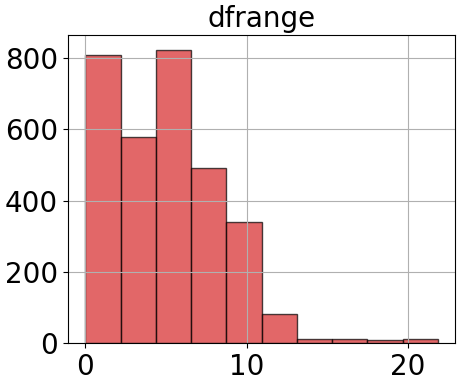
\includegraphics[width=\linewidth]{../../python_code/plots/logistic_regression/histogram-dfrange.png}
    \end{subfigure}
    \begin{subfigure}[t]{.24\textwidth}
        \centering 
        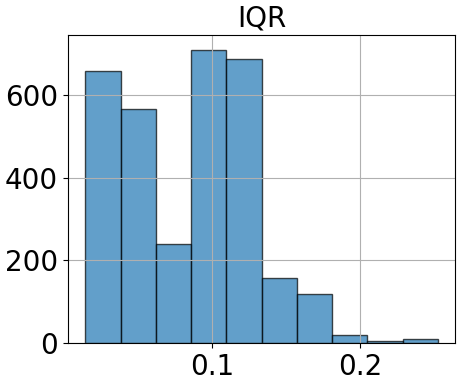
\includegraphics[width=\linewidth]{../../python_code/plots/logistic_regression/histogram-IQR.png}
    \end{subfigure}
    \begin{subfigure}[t]{.24\textwidth}
        \centering 
        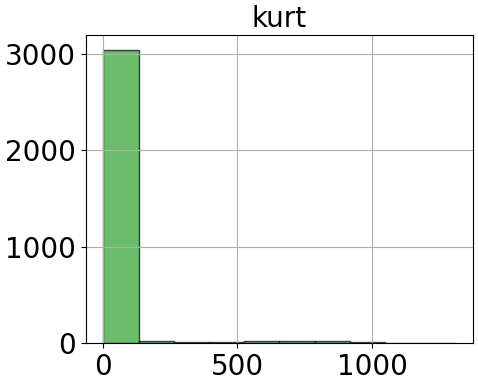
\includegraphics[width=\linewidth]{../../python_code/plots/logistic_regression/histogram-kurt.png}
    \end{subfigure}
% Second row
    \begin{subfigure}[t]{.24\textwidth}
        \centering 
        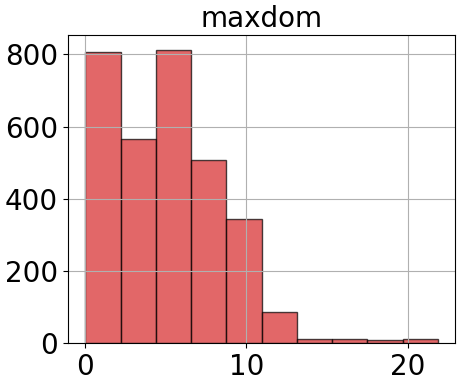
\includegraphics[width=\linewidth]{../../python_code/plots/logistic_regression/histogram-maxdom.png}
    \end{subfigure}
    \begin{subfigure}[t]{.24\textwidth}
        \centering 
        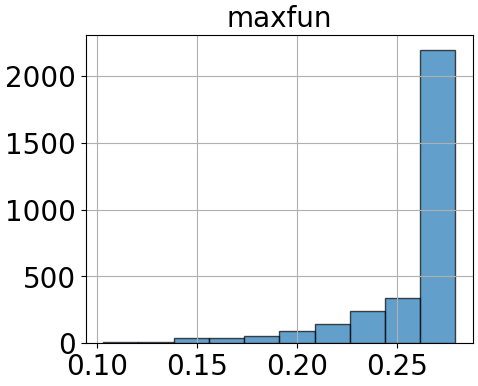
\includegraphics[width=\linewidth]{../../python_code/plots/logistic_regression/histogram-maxfun.png}
    \end{subfigure}
    \begin{subfigure}[t]{.24\textwidth}
        \centering 
        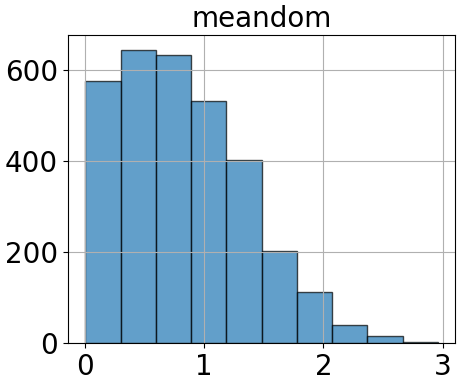
\includegraphics[width=\linewidth]{../../python_code/plots/logistic_regression/histogram-meandom.png}
    \end{subfigure}
    \begin{subfigure}[t]{.24\textwidth}
        \centering 
        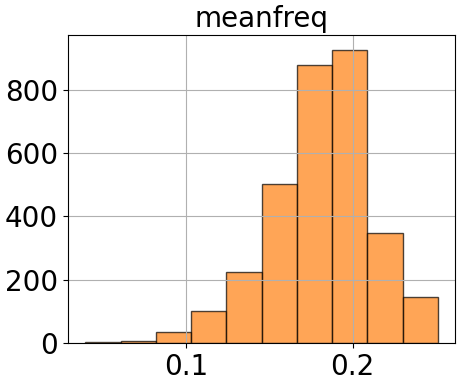
\includegraphics[width=\linewidth]{../../python_code/plots/logistic_regression/histogram-meanfreq.png}
    \end{subfigure}
    \begin{subfigure}[t]{.24\textwidth}
        \centering 
        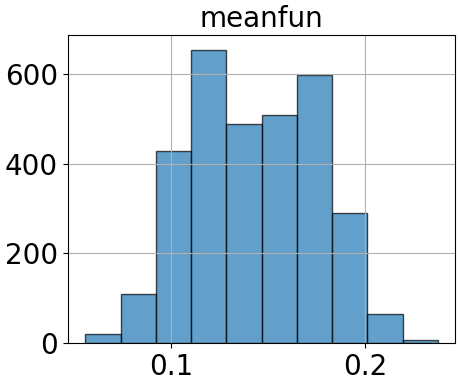
\includegraphics[width=\linewidth]{../../python_code/plots/logistic_regression/histogram-meanfun.png}
    \end{subfigure}
% Third row
    \begin{subfigure}[t]{.24\textwidth}
        \centering 
        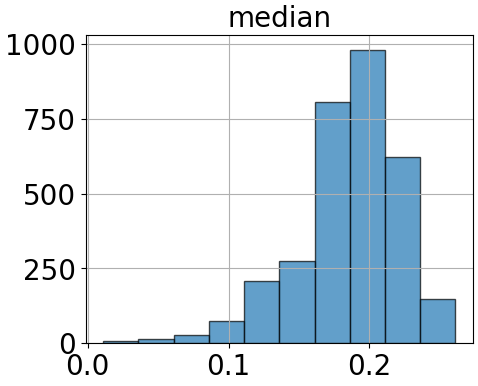
\includegraphics[width=\linewidth]{../../python_code/plots/logistic_regression/histogram-median.png}
    \end{subfigure}
    \begin{subfigure}[t]{.24\textwidth}
        \centering 
        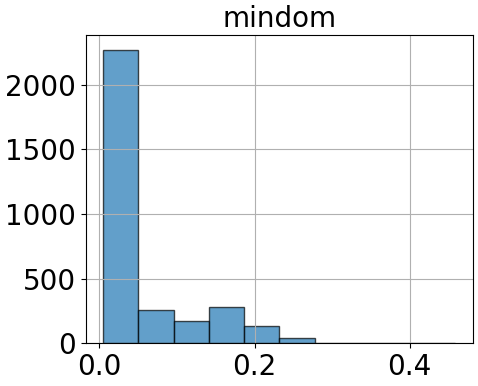
\includegraphics[width=\linewidth]{../../python_code/plots/logistic_regression/histogram-mindom.png}
    \end{subfigure}
    \begin{subfigure}[t]{.24\textwidth}
        \centering 
        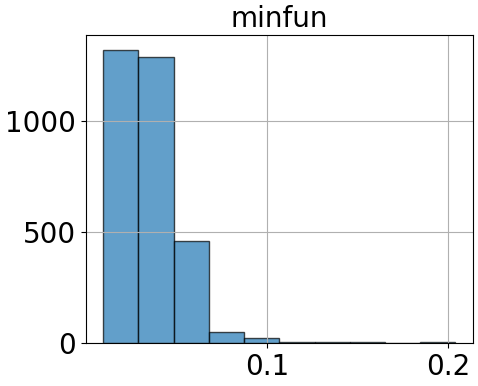
\includegraphics[width=\linewidth]{../../python_code/plots/logistic_regression/histogram-minfun.png}
    \end{subfigure}
    \begin{subfigure}[t]{.24\textwidth}
        \centering 
        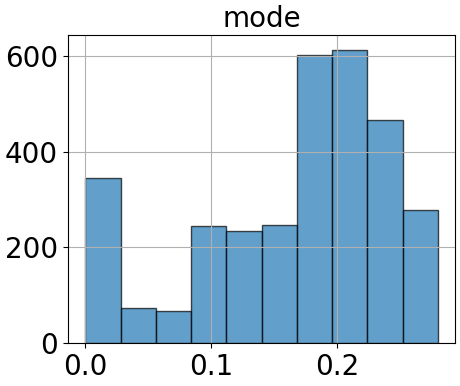
\includegraphics[width=\linewidth]{../../python_code/plots/logistic_regression/histogram-mode.png}
    \end{subfigure}
% Fourth row
    \begin{subfigure}[t]{.24\textwidth}
        \centering 
        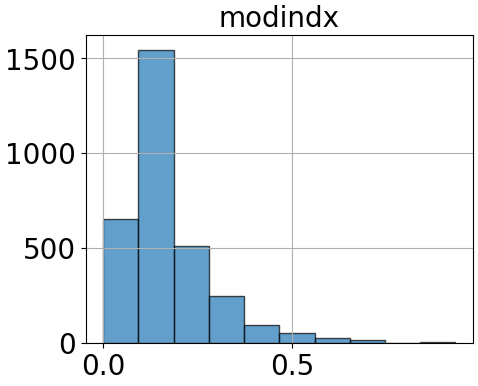
\includegraphics[width=\linewidth]{../../python_code/plots/logistic_regression/histogram-modindx.png}
    \end{subfigure}
    \begin{subfigure}[t]{.24\textwidth}
        \centering 
        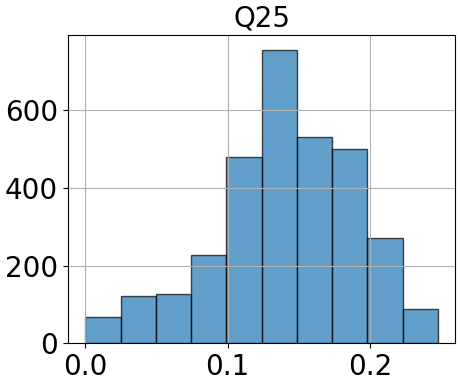
\includegraphics[width=\linewidth]{../../python_code/plots/logistic_regression/histogram-Q25.png}
    \end{subfigure}
    \begin{subfigure}[t]{.24\textwidth}
        \centering 
        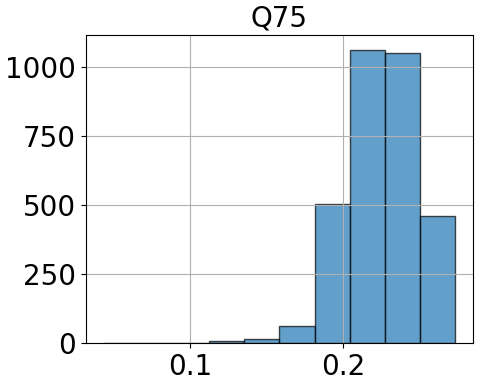
\includegraphics[width=\linewidth]{../../python_code/plots/logistic_regression/histogram-Q75.png}
    \end{subfigure}
    \begin{subfigure}[t]{.24\textwidth}
        \centering 
        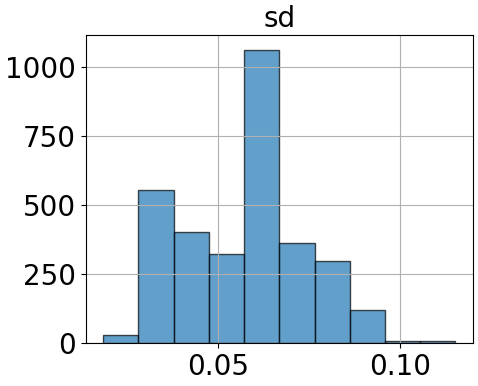
\includegraphics[width=\linewidth]{../../python_code/plots/logistic_regression/histogram-sd.png}
    \end{subfigure}
% Fifth row
    \begin{subfigure}[t]{.24\textwidth}
        \centering 
        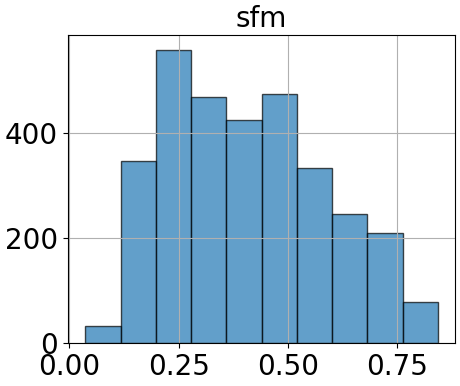
\includegraphics[width=\linewidth]{../../python_code/plots/logistic_regression/histogram-sfm.png}
    \end{subfigure}
    \begin{subfigure}[t]{.24\textwidth}
        \centering 
        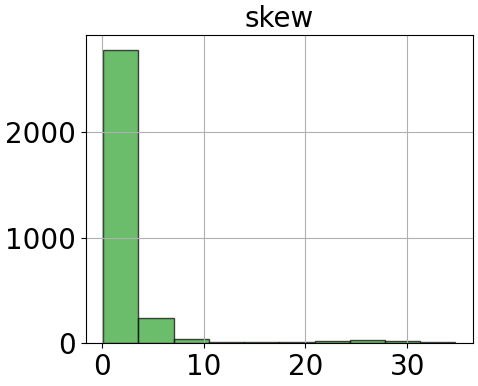
\includegraphics[width=\linewidth]{../../python_code/plots/logistic_regression/histogram-skew.png}
    \end{subfigure}
    \begin{subfigure}[t]{.24\textwidth}
        \centering 
        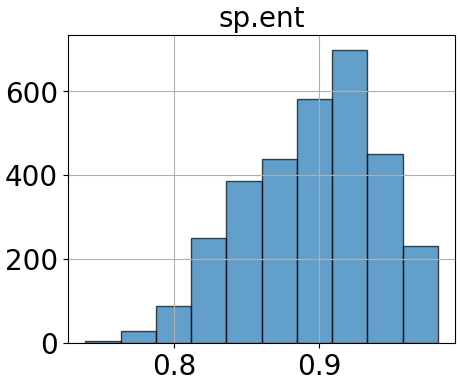
\includegraphics[width=\linewidth]{../../python_code/plots/logistic_regression/histogram-sp.ent.png}
    \end{subfigure}
\end{figure}

The F1-Score and ROC curves below show clearly that 
the regression produces reliable results regardless of threshold value, validating the model.
A threshold of about $0.35$, in particular, 
optimizes the F1-Score in testing while maintaining very high F1-Score in training.
As such, this value is likely to be the most appropriate for this dataset.

For this threshold, the confusion matrix yelded the rates in \cref{fig:confusion-matrix}, 
and overall accuracy of $97.00$\%. 
This was expected because the F1-Score has its second, greatest plateau close to that threshold
and the ROC's associated second point is also close to $97$\% (between $97$\% and $96.9\%$).

\begin{figure}[htbp]
    \centering 
    \caption{
        F1-Score and ROC for (a) training and (b) testing. 
        All rates refer to ``male'' class.
    }
\hfill
    \begin{subfigure}[t]{.33\textwidth}
        \caption{}
        \label{fig:results-training}
        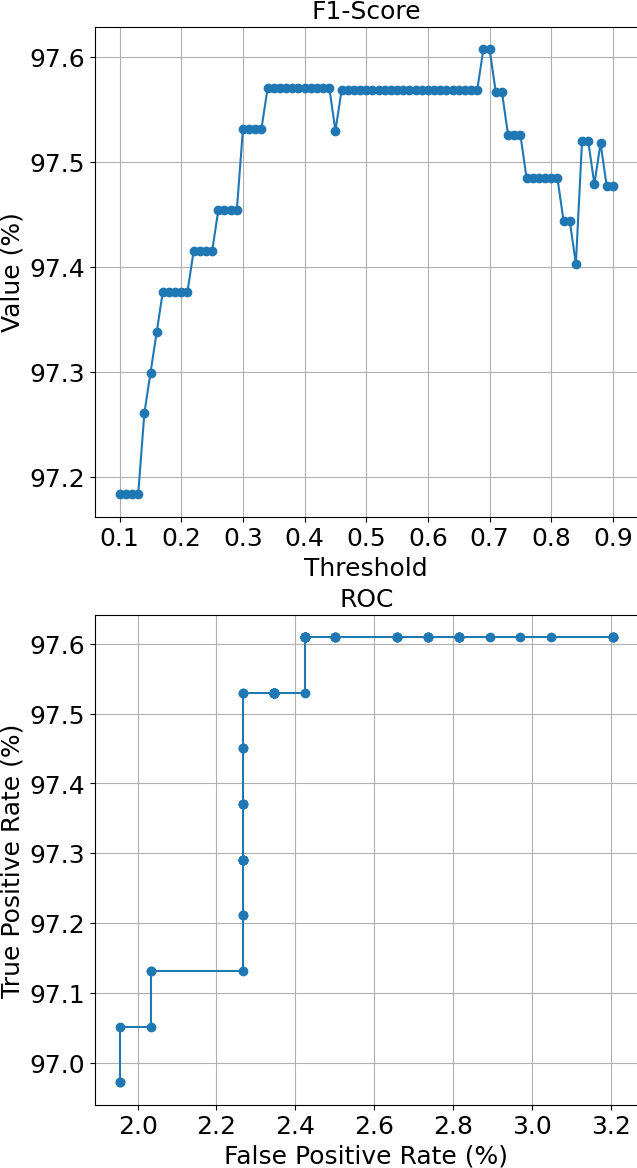
\includegraphics[width=\linewidth]{../../python_code/plots/logistic_regression/results-train.png}
    \end{subfigure}
\hfill
    \begin{subfigure}[t]{.33\textwidth}
        \centering 
        \caption{}
        \label{fig:results-testing}
        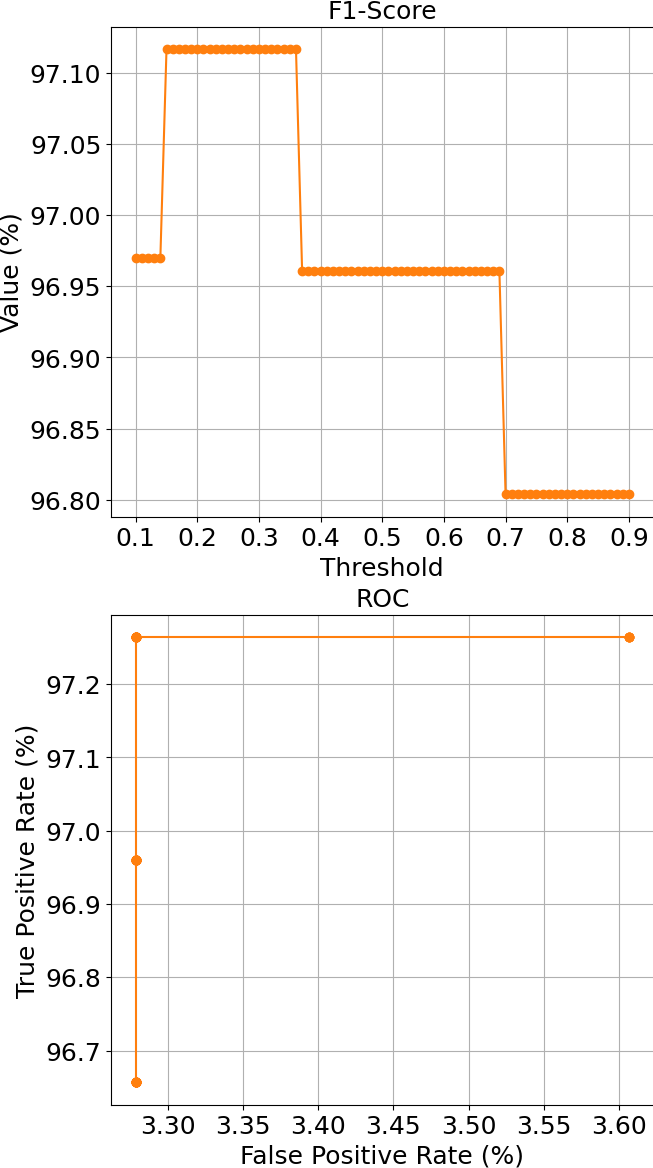
\includegraphics[width=\linewidth]{../../python_code/plots/logistic_regression/results-test.png}
    \end{subfigure}
\hfill\!
\end{figure} 

\begin{figure}[htb]
    \centering 
    \caption{
        Confusion matrix of the regressor using $D=0.35$ in test set.
    }
    \label{fig:confusion-matrix}
    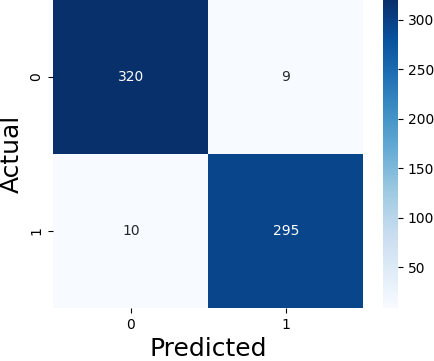
\includegraphics[width=5.5cm]{../../python_code/plots/logistic_regression/results-confusion_matrix.png}
\end{figure} 
